\section{Fitting Decoy Distributions}

The obfuscation of the history of a transaction is a fascinating feature of the Monero blockchain.  
Every transaction is constructed with one or more rings and the real outputs are hidden amongst decoys.
As a physicist, whose colleagues can tease out Higgs Bosons out of a slurry of particles, gravitational waves from the rest of the cosmic background, quantum coherence in a Faraday cage, the idea that one could hide a transaction among decoys, on a graph no-less, was an offensive one to me.  
Yet the decoy selection does seem to introduce enough Fear-Uncertainty-Doubt into a history to achieve the desired outcome of keeping the true history hidden.
It certainly generates a mess while trying to explore and those smart-alecks who do use 300 inputs and 4000+ decoys in a transaction do successfully screech my brute-force approaches to a halt.
However, my suspicions do remain, hence the methodologies conceived herein.

A few things are noteworthy of the implementation of the decoys.  

\begin{itemize}
\item Transactions are held for 10 blocks before they can be reused.  
\item To account for changes in volume that do occur, a dynamic approach is used in selection for the recent transactions.
\item By default, a Gamma Distribution, that has a very thin tail for both long and short times, renders a poor fit for recent times, and makes old transactions in rings rather surprising.
\item Decoys are administered at the wallet level, not the protocol level, and multiple decoy selection algorithms have been deployed in the wild.  Some even repeat entire rings, or otherwise trivialize the detection of the real transaction.  
\item the decoy selection improves with time, but heuristics noted from the past persist through some block range.
\item Methods have gone from static to dynamic and efforts are being made to replace decoys with zero-knowledge proof setups
\end{itemize}

The details for which we are most concerned are the particular values for the probabilities associated with a given element of a given ring.  
We fit a gamma distribution to provide ourselves with a parameterized probability distribution we can subsequently call to determine the filtration parameter we will use in the Persistent Homology by Probability section.
It has been pointed out to me that I used $log(block\, height)$ rather than $log(seconds)$, which could explain the deviation from expectations for the parameter results.  
This error provides a change of scale but not in change of ordering.

The resulting fits are shown for the alpha parameter in \ref{fig:alpha}, \ref{fig:beta}, \ref{fig:fits} below.

\begin{figure}[h]
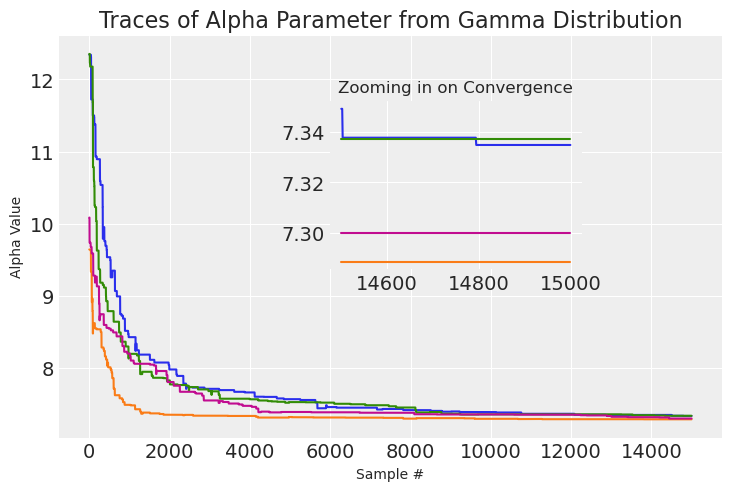
\includegraphics[scale=0.5]{gamma_alpha}
\caption{Fits of the gamma parameter $\alpha$.  Inset zooms in on the region of convergence.}
\label{fig:alpha}
\end{figure}

\begin{figure}[h]
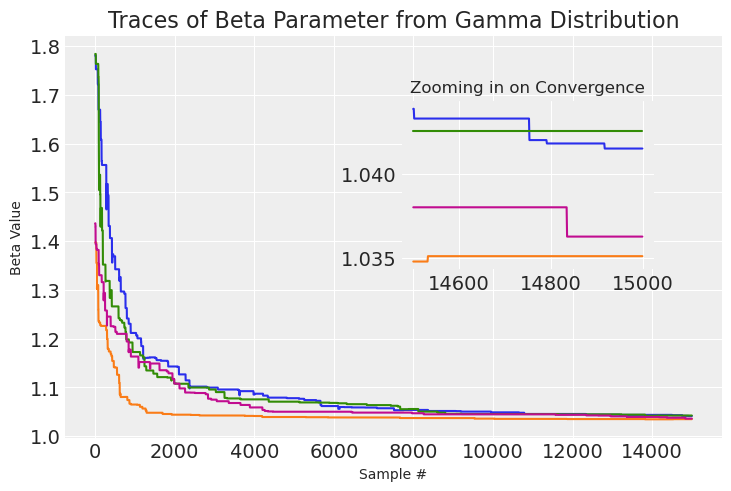
\includegraphics[scale=0.5]{gamma_beta}
\caption{Fits of the gamma parameter $\beta$.  Inset zooms in on the region of convergence.}
\label{fig:beta}
\end{figure}

\begin{figure}[h]
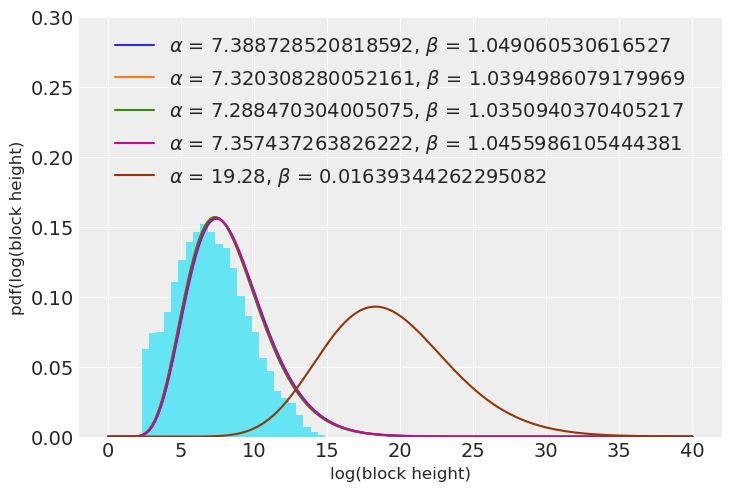
\includegraphics[scale=0.5]{fits}
\caption{The empirical, measured, and theoretical (erratum: wrong scale as described in text)}
\label{fig:fits}
\end{figure}